\chapter{Numerical Experiments}
This chapter is devoted to numerical testing of proposed algorithms. 

\section{Data and Test Environment}
\label{sec:emulator}
All the trials were conducted on synthetic data. Obviously that conducting such experiments on real data is very complicated, however it is on preparation and will be the matter of following studies. 

Here is how testing environment was developed:
\begin{enumerate}
    \item The real mid-January indoor temperatures in a downtown office in Moscow was acquired. 
    \item A dummy Heating Device with three modes (see \ref{fig:matrices_example}) was modelled.
    \item A possible stationery temperatures for each behaviour in each hour were calculated using a simple heat equilibrium model: \todo{insert model}
    \item An ensemble of users was generated. It has the following parameters:
        \begin{itemize}
            \item Comfort temperature $t_0 = 22 C +  \NN(0, 1)$ 
            \item Number of devices $n = 300$
            \item Number of controls $m = 6$
            \item Number of ticks per hour $\tau = 2$
        \end{itemize}
    \item Decision rule: a device accepts a control request if this establish the temperature within $t_0 \pm 2$ and rejects otherwise.
    \item A System Operator was a simple threshold rule which restricts consumption then it reaches $800 \text{ KW/h}$
        
\end{enumerate}

\section{Experimental Results}

Two algorithms from section \ref{sec:algorithms} were to solve \ref{eq:stabilisation_setup} setup on an emulator described above (see section \ref{sec:emulator}). The results were shown on figures: 

Figures displays three graphs: target consumption ({\color{green}green line}), consumption predicted by the algorithm ({\color{orange} orange line}) and real consumption of the ensemble ({\color{blue} blue line}): figure () for PrimalDualBwK algorithm and figure () for liCBwK-m algorithm. One can infer two commonalities for them form these graphs:
\begin{itemize}
    \item Both algorithm are succeeded in consumption stabilising: the average peak-hours demand was decreased in most of the periods. 
    \item Both algorithms are in charge of demand fluctuations in the system which is a significant disadvantage. These oscillations increase of transmission losses and diminish an overall system's stability.
\end{itemize}

On the other hand these algorithms demonstrated at least two distinctions: 
\begin{enumerate}
    \item The \textit{linCBwK-m} algorithm demonstrated better consumption prediction quality. One may assure that in figure \ref{fig:lincbwk_performance} an orange line keeps closer to the blue one, than in figure \ref{fig:pdbwk_performance} while keeping a proper "optimistic" gap. In contrast, the \textit{PrimalDualBwK} demonstrated poorer prediction capabilities and stronger sensitivity to exploration-exploitation performance fluctuations. It is not surprising, as the former algorithm had an embedded ensemble model. However it has shown that such incorporation of physical models to machine learning algorithms has a significant potential in engineering problems. 
    \item Two algorithms treat budget constraints differently: PrimalDualBwK uses semi-greedy strategy of optimal "Bang-per-Buck" ratio, while linCBwK-m uses confidential ellipsoids for estimations of $k(t)$. Consequently, the later algorithm spends the budget more cautiously. In particular, one may see that PrimalDualBwK was out of budget far before the end of the period (see fig. \ref{fig:budget}), which increased his regret as he had to switch to a trivial strategy (see fig. \ref{fig:regret}). In the same time LinCBwK-m spent the budget more deliberately, which allowed him to keep his optimal strategy till the end.
\end{enumerate}
To sum up, the LinCBwK-m algorithm has demonstrated better regret, better prediction capabilities and more intelligent budget expenditure.

\begin{figure}
\centering
\begin{subfigure}{1.1\textwidth}
    \label{fig:pdbwk_performance}
    \centering
    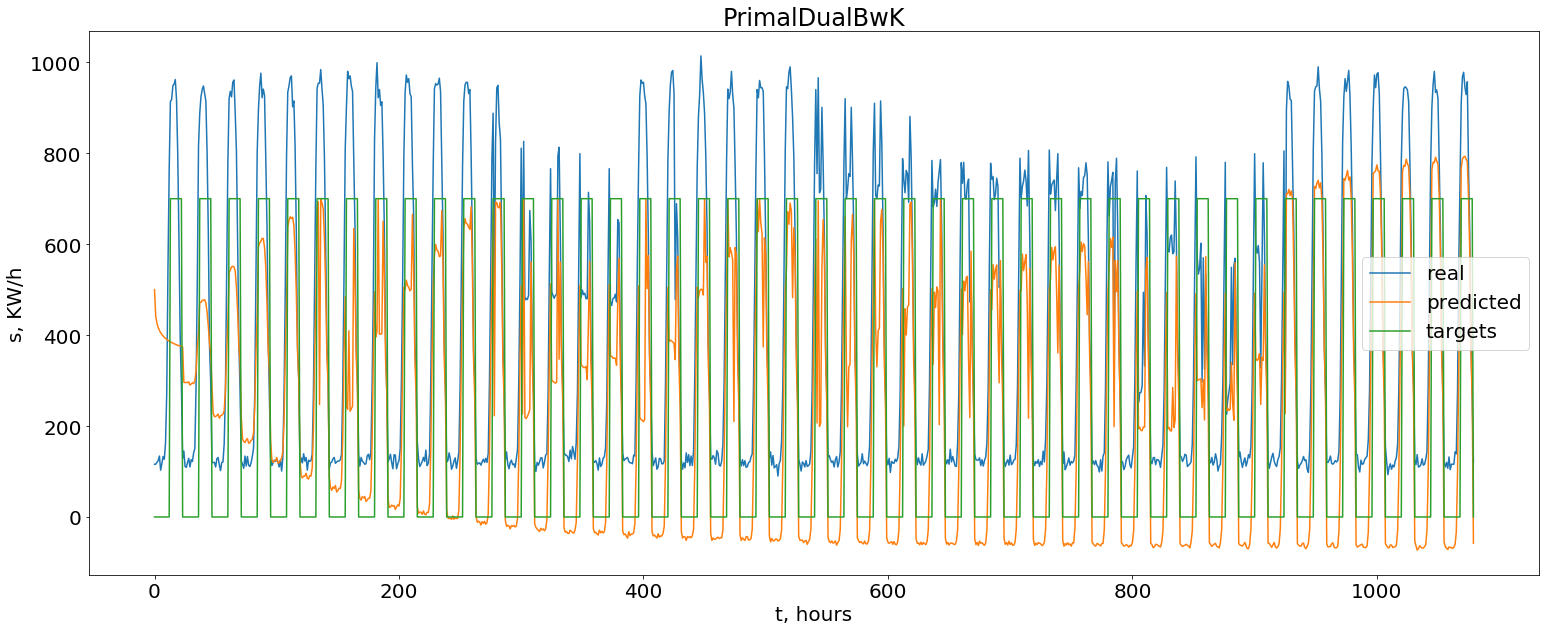
\includegraphics[width=1\textwidth]{figures/pdbwk_consumption}
\end{subfigure}
\begin{subfigure}{1.1\textwidth}
    \label{fig:lincbwk_performance}
    \centering
    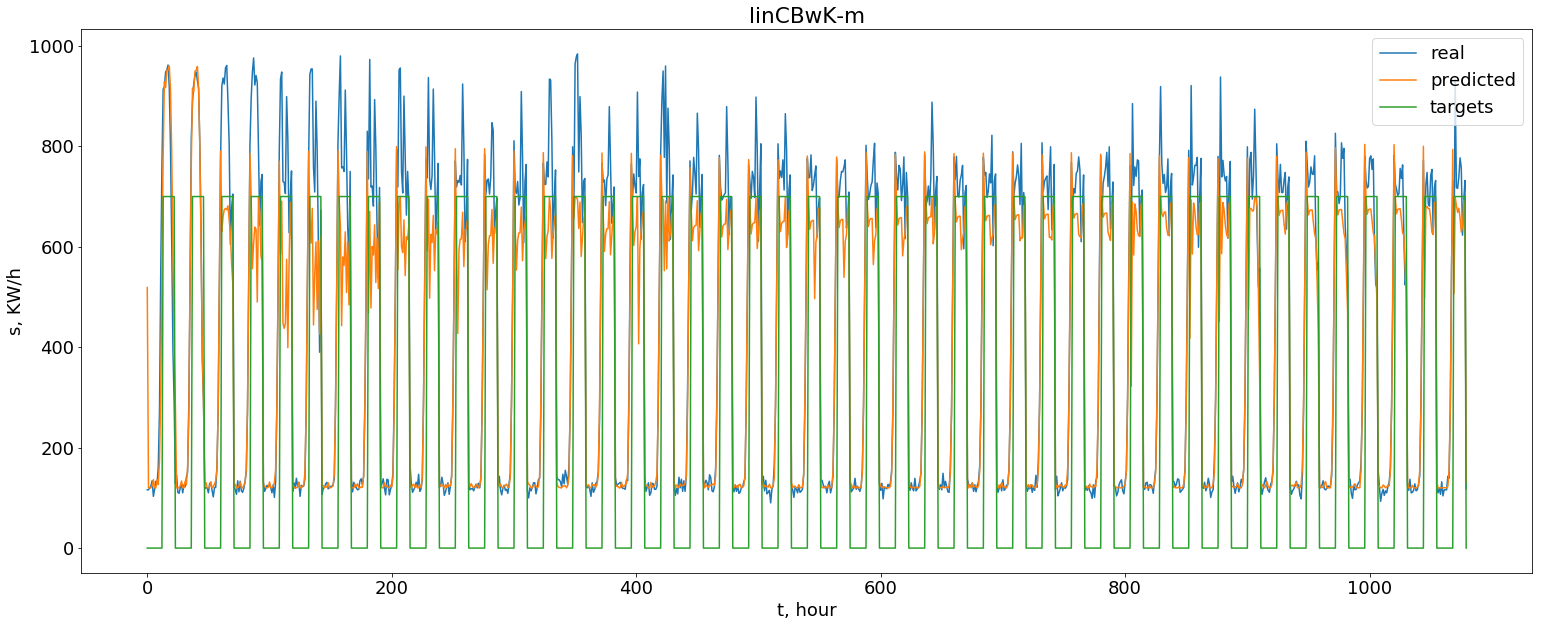
\includegraphics[width=1\textwidth]{figures/lincbwk_consumption}
\end{subfigure}
\caption{Performance comparison of two proposed algorithms: linCBwK-m and PrimalDualBwK. Clearly, the former has better prediction capabilities (orange line keeps close to the blue one), and less sensitive to exploration-exploitation fluctuations.}
\label{fig:performances}
\end{figure}

\begin{figure}
\centering
\begin{subfigure}{.8\textwidth}
    \label{fig:budget}
    \centering
    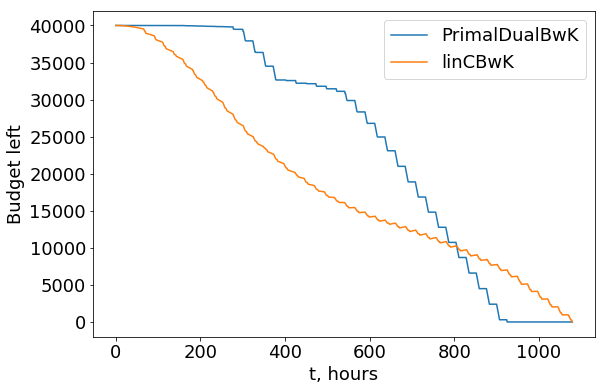
\includegraphics[width=1\textwidth]{figures/budget}
    \caption{Budget expenditure comparison for two proposed algorithms.}
\end{subfigure}
\begin{subfigure}{.8\textwidth}
    \label{fig:regret}
    \centering
    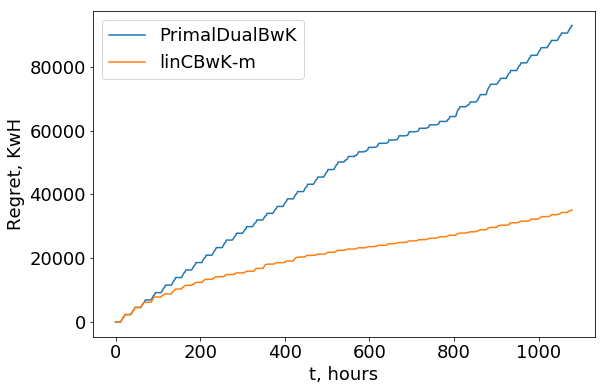
\includegraphics[width=1\textwidth]{figures/regret}
    \caption{Cumulative regret comparison for two proposed algorithms.}
\end{subfigure}
\caption{In this figure cumulative regret curves and budget expenditure curves for two proposed algorithms are shown. The linCBWK algorithm demonstrated significantly better overall performance in comparison to PrimalDualBwK. In addition, the former algorithm demonstrated more cautious budget spending. One may notice, that the later algorithm had all the budget left by 900th hour of online, and had to switch to a trivial strategy (no control). Hence, its regret has soared up after this moment.}
\label{fig:budget_and_regret}
\end{figure}

    